% !TEX TS-program = xelatex
% !TEX encoding = UTF-8
% !Mode:: "TeX:UTF-8"

\documentclass[onecolumn,oneside]{SUSTechHomework}

\usepackage{blindtext}
\usepackage{graphicx}
\usepackage{subfigure}
\usepackage{float}
\usepackage{listings}
\usepackage{hyperref}
\usepackage{algorithm}
\usepackage{algorithmic}
\hypersetup{hidelinks,
	colorlinks=true,
	allcolors=black,
	pdfstartview=Fit,
	breaklinks=true}

\begin{document}
\author{姓名}
\sid{学号}
\title{Latex 常用方法}
\coursecode{xxxx}
\coursename{Introduction to Latex}
\date{Feburary 31, 2012}
\maketitle

\tableofcontents  

\section{插入图片}
\subsection{方法一}
\begin{lstlisting}
  导包:
  \usepackage{graphicx}
  \usepackage{subfigure}
  \usepackage{float}
  代码:
  \begin{figure}[H]
    \centering
    
\includegraphics[scale=0.2]{1.png}
    \caption{你好}
  \end{figure}
\end{lstlisting}
图1:
\begin{figure}[H]
  \centering
  
\includegraphics[scale=0.2]{figures/1.png}
  \caption{你好}
\end{figure}
\subsection{方法二}
\begin{lstlisting}
  \centering
  
\includegraphics[width=7cm,height=4cm]{figures/1.png}
  \caption{你好}
\end{lstlisting}
图2:
\begin{figure}[H]
  \centering
  
\includegraphics[width=7cm,height=4cm]{figures/1.png}
  \caption{你好}
\end{figure}
\section{代码块}
\begin{figure}[H]
  \centering
  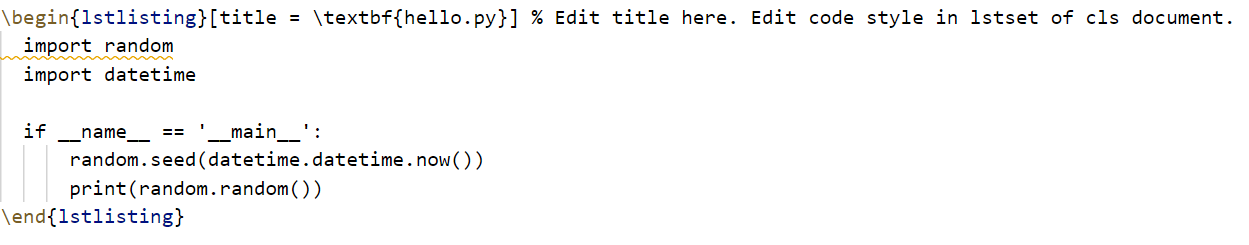
\includegraphics[width=170mm]{figures/2.png}
  \caption{代码块}
\end{figure}
Example:
\begin{lstlisting}[title = \textbf{hello.py}] % Edit title here. Edit code style in lstset of cls document. 
  import random
  import datetime
  
  if __name__ == '__main__':
      random.seed(datetime.datetime.now())
      print(random.random())
\end{lstlisting}

\section{排版}
\subsection{段落}
Four score and seven years ago our fathers brought forth on this continent, 
a new nation, conceived in Liberty, and dedicated to the proposition that 
all men are created equal. \par

Now we are engaged in a great civil war, testing whether that nation, 
or any nation so conceived and so dedicated, can long endure. 
We are met on a great battle-field of that war. We have come to dedicate 
a portion of that field, as a final resting place for those 
who here gave their lives that that nation might live. 
It is altogether fitting and proper that we should do this.\par
\subsection{空行}
\begin{lstlisting}
  \vspace*{n\baselineskip}
  \\
  \newline
  \par
\end{lstlisting}
1============================\par
\vspace*{1\baselineskip} 
1============================\par
2============================\par
\vspace*{2\baselineskip} 
2============================
\subsection{换页}
\begin{lstlisting}
  \thispagestyle{empty}
\end{lstlisting}
\subsection{页码}
\begin{lstlisting}
  \setcounter{page}{1}  从此页开始1 2 3
  \thispagestyle{empty} 此页无页码
\end{lstlisting}
\subsection{目录}
\begin{lstlisting}
  \tableofcontents  
\end{lstlisting}
\subsection{列表}
\subsubsection{参考链接:}
\begin{lstlisting}
  导包:
  \hypersetup{hidelinks,
	colorlinks=true,
	allcolors=blue,
	pdfstartview=Fit,
  breaklinks=true}
  代码:
  \href{https://www.cnblogs.com/ahhylau/p/4586167.html}{https://www.cnblogs.com/ahhylau/p/4586167.html}
\end{lstlisting}
\href{https://www.cnblogs.com/ahhylau/p/4586167.html}{https://www.cnblogs.com/ahhylau/p/4586167.html}
\subsubsection{案例}
\begin{lstlisting}
  \begin{enumerate}
    \item This is the first item
    \begin{enumerate}
      \item sub1
      \item sub2
    \end{enumerate}
    \item This is the second item
    \item This is the third item
  \end{enumerate}
  \begin{itemize}
    \item This is the first item
    \begin{itemize}
      \item sub1
      \item sub2
      \item sub3
    \end{itemize}
    \item This is the second item
    \item This is the third item
  \end{itemize}
\end{lstlisting}
\begin{enumerate}
  \item This is the first item
  \begin{enumerate}
    \item sub1
    \item sub2
  \end{enumerate}
  \item This is the second item
  \item This is the third item
\end{enumerate}
\begin{itemize}
  \item This is the first item
  \begin{itemize}
    \item sub1
    \item sub2
    \item sub3
  \end{itemize}
  \item This is the second item
  \item This is the third item
\end{itemize}
\section{公式}
\subsection{行内公式}
\begin{lstlisting}
  $公式$
\end{lstlisting}
我们知道:$\theta=2\pi$, $\therefore$ proof is right.
\subsection{行间公式}
\begin{lstlisting}
  $$
  公式
  $$
\end{lstlisting}
狗屁不通的定理:
$$
\theta*\gamma=\gamma*\alpha
$$
\section{表格}
\href{https://www.tablesgenerator.com/}{在线生成表格} \par
\href{https://zhuanlan.zhihu.com/p/62317790}{知乎讲解}
\begin{lstlisting}
  \begin{table}[H]
    \begin{tabular}{|l|l|l|l|l|}
    \hline
     A&1  &2  &3 &4  \\ \hline
     B&5 &6  &7  &8  \\ \hline
     C&9  &10  &11  &12  \\ \hline
     D&13  &14  &15  &16  \\ \hline
    \end{tabular}
  \end{table}  
\end{lstlisting}
\begin{table}[H]
  \begin{tabular}{|l|l|l|l|l|}
  \hline
   A&1  &2  &3 &4  \\ \hline
   B&5 &6  &7  &8  \\ \hline
   C&9  &10  &11  &12  \\ \hline
   D&13  &14  &15  &16  \\ \hline
  \end{tabular}
\end{table}
\section{文本框}
\begin{lstlisting}
\begin{center}
\fcolorbox{black}{gray!5}{
\parbox{1\linewidth}{
  The first Line.\\
  The second Line.\\
  $\theta=A*B$      
}
}
\end{center}
\end{lstlisting}
\begin{center}
		\fcolorbox{black}{gray!5}{
      \parbox{1\linewidth}{
        The first Line.\\
        The second Line.\\
        $\theta=A*B$
      }
		}
\end{center}
\section{Algorithm}
\begin{lstlisting}[title = \textbf{Algorithm Design}]
  \begin{algorithm}
    \caption{Calculate $y = x^n$}
    \label{alg1}
    \begin{algorithmic}
    \REQUIRE $n \geq 0 \vee x \neq 0$
    \ENSURE $y = x^n$
    \STATE $y \leftarrow 1$
    \IF{$n < 0$}
    \STATE $X \leftarrow 1 / x$
    \STATE $N \leftarrow -n$
    \ELSE
    \STATE $X \leftarrow x$
    \STATE $N \leftarrow n$
    \ENDIF
    \WHILE{$N \neq 0$}
    \IF{$N$ is even}
    \STATE $X \leftarrow X \times X$
    \STATE $N \leftarrow N / 2$
    \ELSE[$N$ is odd]
    \STATE $y \leftarrow y \times X$
    \STATE $N \leftarrow N - 1$
    \ENDIF
    \ENDWHILE
    \end{algorithmic}
  \end{algorithm}
\end{lstlisting}
\begin{algorithm}
  \caption{Calculate $y = x^n$}
  \label{alg1}
  \begin{algorithmic}
  \REQUIRE $n \geq 0 \vee x \neq 0$
  \ENSURE $y = x^n$
  \STATE $y \leftarrow 1$
  \IF{$n < 0$}
  \STATE $X \leftarrow 1 / x$
  \STATE $N \leftarrow -n$
  \ELSE
  \STATE $X \leftarrow x$
  \STATE $N \leftarrow n$
  \ENDIF
  \WHILE{$N \neq 0$}
  \IF{$N$ is even}
  \STATE $X \leftarrow X \times X$
  \STATE $N \leftarrow N / 2$
  \ELSE[$N$ is odd]
  \STATE $y \leftarrow y \times X$
  \STATE $N \leftarrow N - 1$
  \ENDIF
  \ENDWHILE
  \end{algorithmic}
\end{algorithm}
\section{一些特别好用的网站}
\begin{itemize}
  \item 模板:
  \begin{itemize}
    \item \href{http://www.latextemplates.com/}{http://www.latextemplates.com/}
    \item \href{https://www.overleaf.com/latex/templates/}{https://www.overleaf.com/latex/templates/}
  \end{itemize}
  \item Latex 常用公式总结:
  \begin{itemize}
    \item \href{https://blog.csdn.net/GarfieldEr007/article/details/51646604}{https://blog.csdn.net/GarfieldEr007/article/details/51646604}
    \item \href{https://www.moonpapers.com/manual/latex/}{https://www.moonpapers.com/manual/latex/}
  \end{itemize}
\end{itemize}
\section{IDE 的选择}
\begin{figure}[H]
  \centering
  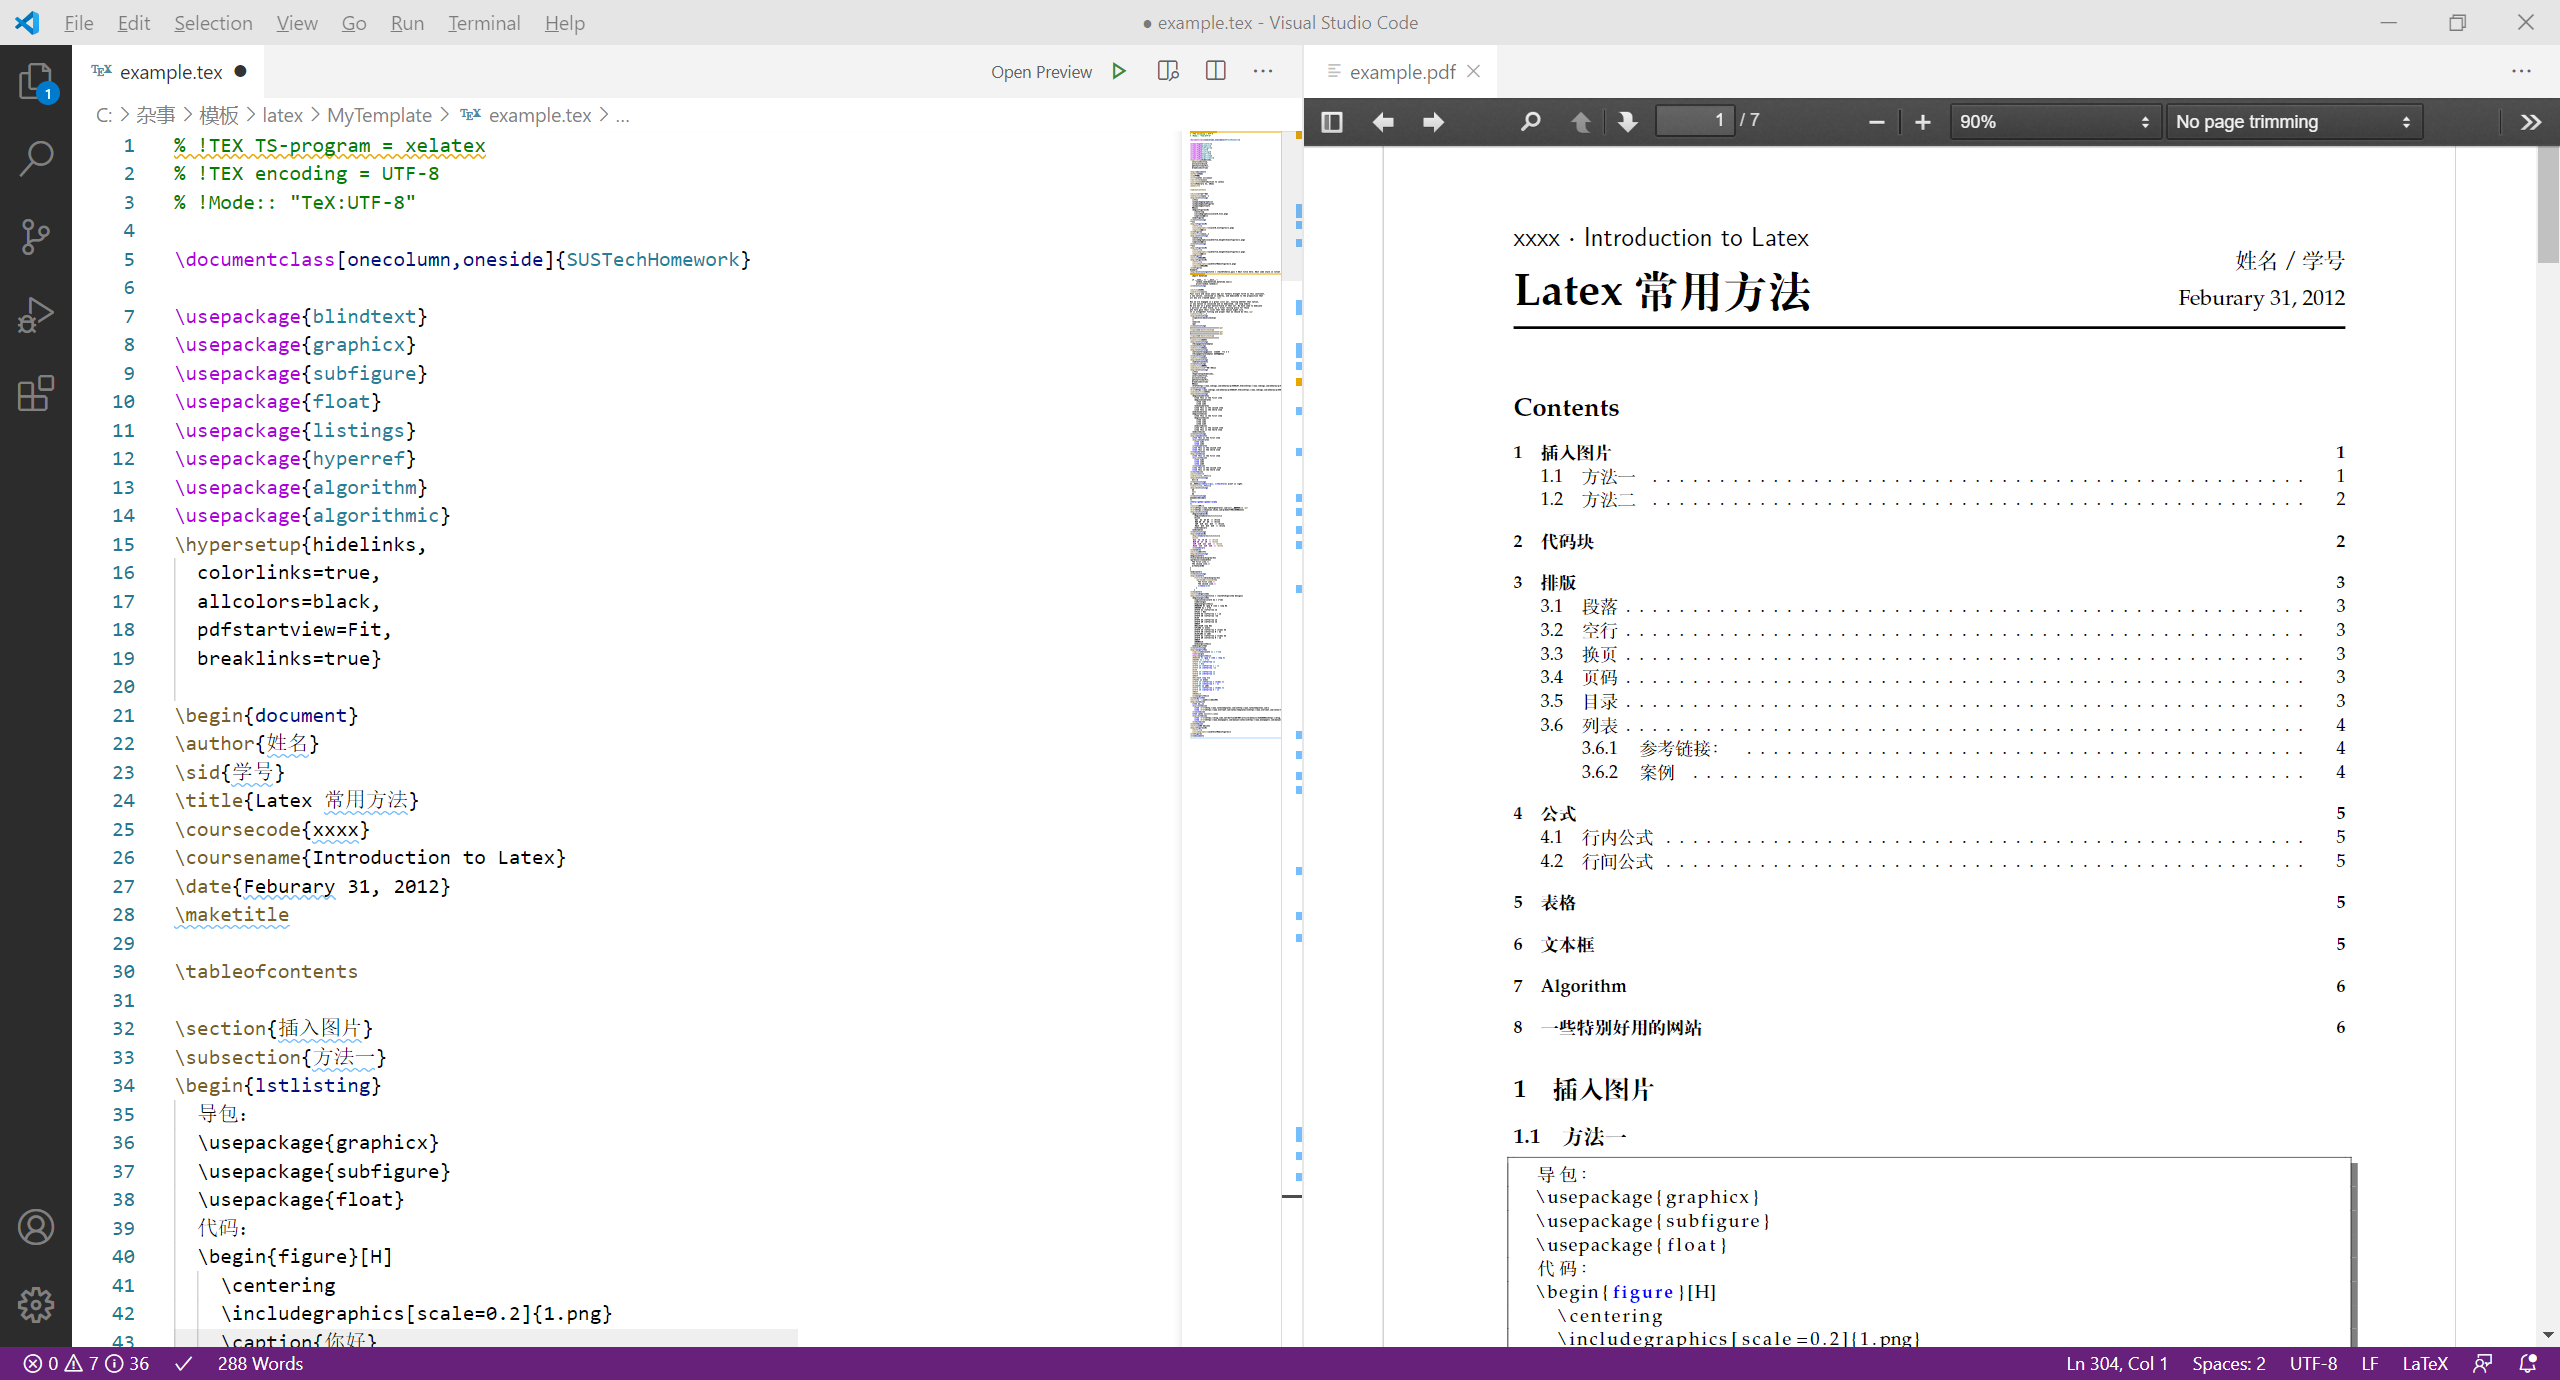
\includegraphics[width=170mm]{figures/3.png}
\end{figure}
\begin{itemize}
  \item 不得不说,vscode十分好用。(代码提示+代码补全+英语语法纠错)
  \item 需要的插件:
  \begin{figure}[H]
    \centering
    
\includegraphics[width=170mm]{figures/4.png}
  \end{figure}
\end{itemize}
\section{致谢}
本文采用了\textbf{\href{https://github.com/ziqin/LaTeX-SUSTechHomework}{学长提供的通用模板}}并略作修改,在此表示衷心的感谢。
\end{document}
